% Формат бумаги: А4.
\documentclass[a4paper]{report}
\usepackage[utf8]{inputenc}
\usepackage[russian]{babel}
\usepackage{amsmath,amsfonts,amssymb,cite,url,verbatim,graphicx,wrapfig}
\graphicspath{{images/}}
\usepackage{booktabs}
\usepackage{graphicx}
\usepackage{array}
\usepackage{relsize}

% Поля: верхнее – 2 см, нижнее – 2 см, левое – 3 см, правое – 1.5 см.
\usepackage{geometry}
\geometry{
	left = 3cm,
	top = 2cm,
	right = 1.5cm,
	bottom = 2cm
}


%\setlength{\parindent}{1.5cm}

% Кегль: основной текст – 14 пт, названия параграфов – 16 пт, названия глав – 18 пт, текст в таблице, подписи к рисункам, таблицам – 12 пт.
\renewcommand{\small}{\fontsize{12}{12}\selectfont}
\renewcommand{\normalsize}{\fontsize{14}{14}\selectfont}
\renewcommand{\large}{\fontsize{16}{16}\selectfont}
\renewcommand{\Large}{\fontsize{18}{18}\selectfont}
\renewcommand{\huge}{\fontsize{20}{20}\selectfont}
\usepackage{sectsty}
\sectionfont{\Large}
\subsectionfont{\large}
\paragraphfont{\normalsize}
\usepackage[font=small]{caption}

% Межстрочный интервал: 1.5 строки.
\usepackage{setspace}
\linespread{1.5}

% Абзацный отступ. Первая строка каждого абзаца должна иметь абзацный отступ 1.25 см.
\usepackage{indentfirst}
\setlength{\parindent}{1.25cm}

% Выравнивание основного текста по ширине поля.
\usepackage{ragged2e}
\justifying

%%% здесь лучше ничего не трогать
\setcounter{tocdepth}{2}
\renewcommand{\thesection}{}
\renewcommand{\thesubsection}{}
\allsectionsfont{\centering}
\usepackage{titlesec}
\newcommand{\sectionbreak}{\clearpage}
\usepackage{tocloft}
\cftsetindents{section}{0em}{0em}
\cftsetindents{subsection}{2em}{0em}
\AtBeginDocument{\renewcommand{\contentsname}{\begin{center} \vskip-2.5cm \Large{Содержание} \end{center}}}
\AtBeginDocument{\renewcommand{\bibname}{}}
%%%

\begin{document}
	%%%%% TITLE PAGE %%%%%
\thispagestyle{empty}
\begin{center}
\textsc{Санкт-Петербургский государственный университет \\
\textbf{Кафедра технологий программирования}} \\
\vspace{1cm}
\Large{\textbf{Башарин Егор Валерьевич}} \\
\vspace{1cm}
\large{\textbf{Выпускная квалификационная работа бакалавра}} \\ 
\vspace{2cm}
\Large{\textbf{Контекстная обработка данных социальных сетей}} \\ 
\normalsize{Направление 010400 \\
Прикладная математика и информатика} \\
\end{center}
\vspace{2cm}
\hspace{9cm} Научный руководитель, \\
\hspace*{9cm} старший преподаватель \\
\hspace*{9cm} Попова С.В. 
\begin{center}
\vfill
Санкт-Петербург \\
2016
\end{center}
	\newpage
	
	%%%%% CONTENTS %%%%%
	\tableofcontents
	\newpage
	
	
%%%%%%%%%%%%%%%%%%%%%%%%%%%%%%%%%%%%%%%%%%%%%%%%%%%%%%%
%%%%%%%%%%%%%%%%%%%%%%%%%%%%%%%%%%%%%%%%%%%%%%%%%%%%%%%
                   %%%%% Intro %%%%%
%%%%%%%%%%%%%%%%%%%%%%%%%%%%%%%%%%%%%%%%%%%%%%%%%%%%%%%
%%%%%%%%%%%%%%%%%%%%%%%%%%%%%%%%%%%%%%%%%%%%%%%%%%%%%%%
	\section{Введение} 
	В настоящее время явление социальных сетей достаточно распространено. Социальные сети уверенно вошли в жизнь современного человека и теперь занимают в ней значимую часть. Главным образом они оказывают влияние на поведение, предубеждения, ценности и намерения человека, что отражается во всех сферах его деятельности. Оказываемое влияние, быстрый рост популярности и открытый доступ к контенту привлекли к социальным сетям внимание правительства, финансовых организаций и исследователей. 
	%Преобразование контента социальных сетей в текстовую информацию и
	Выделение ключевых концепций стало важным условием для порождения знаний и формулирования стратегий. Анализ полученных данных помогает исследователям улучшить понимание об информационных потоках, о формировании и распространении мнений, о связи ценностей и предубеждений пользователя и генерируемого им контента. 
	%Тем не менее число качественных и количественных исследований в данной области слишком мало. 
	Существенным барьером при использовании социальных сетей является необходимость выбора методологии для сбора, обработки и анализа информации, полученной с сайтов социальных сетей. Однако, существуют компании по производству программного обеспечения, разрабатывающие проприетарные системы сбора информации для визуализации данных, и исследователи, занимающиеся разработкой экспертных систем для анализа настроений \cite{bib:Kaklauskas}. 
	
Пользователи социальных сетей ежедневно публикуют данные о своей активности, чувствах и мыслях, выражая свое мнение и позицию. Это способствует появлению в социальных сетях групп пользователей (сообществ), имеющих общие интересы. Для выявления ключевых концепций и тематик присущих группе пользователей используется контекстная обработка  генерируемого ими контента. В данной работе контекстная обработка данных основана на идеях и принципах тематического моделирования. Результаты такой обработки могут использоваться для мониторинга мнений и политических взглядов пользователей или для предсказания поведения рынка. \\

%%%%%%%%%%%%%%%%%%%%%%%%%%%%%%%%%%%%%%%%%%%%%%%%%%%%%%%
%%%%%%%%%%%%%%%%%%%%%%%%%%%%%%%%%%%%%%%%%%%%%%%%%%%%%%%
                   %%%%% Постановка задачи %%%%%
%%%%%%%%%%%%%%%%%%%%%%%%%%%%%%%%%%%%%%%%%%%%%%%%%%%%%%%
%%%%%%%%%%%%%%%%%%%%%%%%%%%%%%%%%%%%%%%%%%%%%%%%%%%%%%%
	 
	\section{Постановка задачи}
	Целью данной работы является изучение методов контекстной обработки данных социальных сетей, в основе которых лежат при принципы и идеи тематического моделирования. Стоит обратить внимание, что под социальной сетью в данной работе понимается веб-сайт или онлайн-сервис, который предназначен для поддержания социальных взаимоотношений при помощи Интернета. 
	 Для того чтобы достичь поставленной цели предлагается выполнить следующий ряд задач:
	
	
	\renewcommand{\labelenumi}{\arabic{enumi}.}
	\renewcommand{\labelenumii}{\arabic{enumi}.\arabic{enumii}}

	\begin{enumerate}
	\item{Выбор источника данных}
		\begin{enumerate}
		\item{Обзор социальных сетей}
		\item{Выбор социальной сети}
		\end{enumerate}
	\item{Подготовка данных}
		\begin{enumerate}
		\item{Загрузка данных с веб-страниц социальной сети}
		\item{Предварительная обработка данных}
		\item{Разбиение данных на обучающую и тестовую части}
		\end{enumerate}
	\item{Выбор тематической модели}
		\begin{enumerate}
		\item{Анализ тематических моделей}
		\item{Выбор подходящей тематической модели}
		\end{enumerate}
	\item{Построение тематической модели}
		\begin{enumerate}
		\item{Анализ методов построения тематической модели}
		\item{Реализация программного модуля, реализующего выбранную тематическую модель}
		\item{Обучение тематической модели}
		\end{enumerate}
	\item{Оценка качества модели}
		\begin{enumerate}
		\item{Обзор и анализ оценок качества тематических моделей}
		\item{Оценка качества построенной модели}
		\end{enumerate}
	\item{Анализ полученных результатов}
	\end{enumerate}

%%%%%%%%%%%%%%%%%%%%%%%%%%%%%%%%%%%%%%%%%%%%%%%%%%%%%%%
%%%%%%%%%%%%%%%%%%%%%%%%%%%%%%%%%%%%%%%%%%%%%%%%%%%%%%%
                   %%%%% Обзор литературы %%%%%
%%%%%%%%%%%%%%%%%%%%%%%%%%%%%%%%%%%%%%%%%%%%%%%%%%%%%%%
%%%%%%%%%%%%%%%%%%%%%%%%%%%%%%%%%%%%%%%%%%%%%%%%%%%%%%%
	\section{Обзор литературы}
	
	Тема данной работы тесно пересекается с информационным поиском, основы которого подробно рассмотрены в книге Кристофера Майнинга "Introduction to Information Retrieval" \cite{bib:InformationRetrieval}. Особое внимание стоит уделить главам 2 и 18. В главе~2 описываются методы подготовки и предварительной обработки текстовой информации. Глава~18 сосредотачивает внимание на подходах латентно-семантического анализа, который является ценным инструментом в тематическом моделировании. В конце каждой главы приведены ссылки на литературу для более подробного изучения темы. 
	
	Вероятностное латентно-семантическое моделирование стало логичным продолжением идей латентно-семантического моделирования и нашло свое применение в тематическом моделировании. Это стало причиной появления вероятностных тематических моделей. Основные принципы вероятностного латентно-семантического анализа (probabilistic latent semantic analysis - pLSA) были описаны Томасом Хоффманом в 1999 году в статье \cite{bib:Hoffman}. Затем они были развиты Дэвидом Блеем в его статье 2003 года \cite{bib:Blei}, в которой была введена и рассмотрена тематическая модель латентного размещения Дирихле (latent dirichlet allocation - LDA). Статья Д.Блея описывает основные преимущества LDA перед pLSA, а также методы построения и оценки качества тематической модели LDA. В статье Д.Блея 2012 года \cite{bib:Blei2} рассматриваются связь LDA с другими вероятностными тематическими моделями, а также применение LDA в тематическом моделировании.
	
	В техническом отчете Грегора Хейнрича "Parameter estimation for text analysis" \cite{bib:Heinrich}  рассматриваются методы оценки параметров моделей для тематического анализа текстов. В отчете подробно разобраны темы, связанные с основными подходами оценки параметров, сопряженными распределениями и Байесовскими сетями, а также применение данных тем для построения тематической модели LDA. 
	
	 Среди русскоязычной литературы следует обратить внимание на работы К.~В.~Воронцова.  В работе \cite{bib:Voron1} подробно описаны основные идеи вероятностного тематического моделирования. В первой части данной работы ставится задача тематического моделирования. Далее рассматриваются основные вероятностные тематические модели pLSA, LDA и их модифицированные версии, а также методы их построения. Работа завершается рассмотрением способов оценки качества тематических моделей.
	

	
	
	
	\section{Глава 1. Подготовка данных}
	\subsection{1.1 Обзор социальных сетей}
	
	
	
	Несмотря на то, что социальные сети появлись около 20 лет назад, их популярность растет с каждым годом. На рисунке \ref{fig:popularity}  показан график, отображающий рост числа пользоватлей социальных сетей во всем мире. По итогам 2015 года число пользователей социальных сетей превысило отметку в 2 миллиарда человек и по прогнозам их количество будет только расти \cite{bib:Popularity}. В соответсвии с этим можно сделать вывод о том, что социальные сети прочно укрепляются в жизни совеременного человека, а их изучение становится актуальной проблемой.
	\newline
	\newline
	\begin{figure}[h]
		
		\centering
		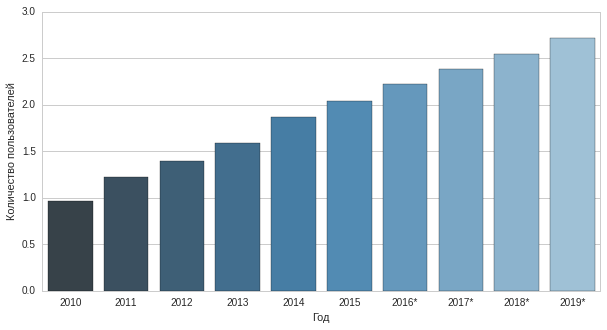
\includegraphics[width=400px]
		{imgs/Popularity.png}
		\caption{Число пользователей социальных сетей по годам}
		\label{fig:popularity}
	\end{figure}
	\newline			
	\newline
	
	
	
	Число социальных сетей довольно велико, и каждая из них предоставляет различные возможности для пользователей и преследует различные цели.  На рисунке \ref{fig:stat} представлен график, отражающий количество активных пользователей в самых популярных социальных сетях на апрель 2016~года  \cite{bib:PopularNetwork}. На графике видно, что такие социальные сети как Facebook, WhatsApp, Facebook messenger и QQ пользуются наибольшей популярностью у пользователей. 	
	Также стоит обратить внимание на социальную сеть VKontakte, которая довольно популярна в российском сегменте интернета и насчитывает около 100 миллионов активных пользователей.
	
	Социальные сети Facebook и Vkontakte предоставляют похожие возможности своим пользователям: создание профиля с фотографией и информацией о себе, обмен сообщениями с другими пользователями, публикация сообщений на страницах других пользователей или сообществ, создание сообществ, загрузка видеозаписей и фотографий и множество других функций для взаимодействия между пользователями. Такие социальные сети как WhatsApp, QQ, WeChat, Skype, Viber, Telegram в основном выполняют роль месседжеров и их предназначенение ограничивается обменом текстовой, аудио- и видео- информации между пользователями. Социальная сеть Instagram в основном ориентирована на публикацию пользователями фотографий и видеозаписей.
	%предоставляет своим пользователям возможности обмена фотографиями и видеозаписями. 
	Особенность социальной сети Twitter - это возможность публикации коротких сообщений. Linkedin представляет собой социальную сеть, предназначенную для поиска и установления деловых связей.
	
	
	
	
	


	
	\begin{figure}
		\centering
		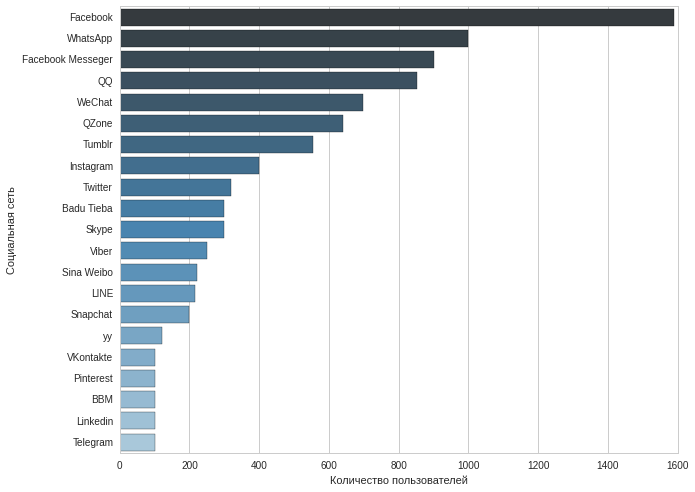
\includegraphics[width=400px]
		{imgs/NetworkStatistics.png}
		\caption{Рейтинг самых популярных  социальных сетей на апрель 2016 года}
		\label{fig:stat}
	\end{figure}
	
	
	
	
	
	\subsection{1.2 Выбор социальной сети и загрузка данных}
	
	В качестве исходных данных рассмотрим публикации в сообществах социальных сетей. 
	Такие сообщества, как правило, представляют собой одну или несколько веб-страниц. 
	Каждое сообщество обладает определенной тематической направленностью: спорт, музыка, политика, финансы и~др.
	Возможность создания сообществ поддерживается такими социальными сетями как Facebook и Vkontakte. 
	В данной работе рассматривается социальная сеть Vkontake, так как она наиболее популярна в российском сегменте интернета.
			
	
	Для того чтобы загрузить публикации из сообществ социальной сети Vkontakte был реализован программный модуль на языке программирования Python~2.7. 
	Для получения доступа к информации о сообществах и их публикациям использовалась технология API~Vkontakte \cite{bib:vkapi}, которая предоставляет методы для работы с данными социальной сети \cite{bib:methods}. Число обращений к методам API имеет ограничение: не более 3 раз в секунду.
	
	API (Application programming interface, интерфейс программировния приложений) представляет собой набор готовых классов, функций и структур, предоставляемых сервисом для использования во внешних программных продуктах. 
	
	Для загрузки данных реализованный программный модуль делает запросы к методам API Vkontakte для выполнения следующих задач:
	
	%\renewcommand{\labelenumi}{\arabic{enumi}.}
	%\renewcommand{\labelenumii}{\arabic{enumi}.\arabic{enumii}}
	\begin{enumerate}
	\item{Получение информации о категориях сообществ с помощью метода API <<groups.getCatalogInfo>>}
	\item{Получение списка популярных сообществ для каждой категории с помощью метода API <<groups.getCatalog>> }
	\item{Получение публикаций для каждого сообщества с помощью метода API <<wall.get>>}
	
	\end{enumerate}
	
	\setlength\extrarowheight{5pt}
\begin{table}[t]
\centering
\begin{tabular}{|c|c|}
\hline
\textbf{Идентификатор категории} & \textbf{Название категории} \\  \hline 
0 & Рекомендации \\ \hline
1 & Новости \\ \hline
2 & Спорт \\ \hline
3 & Музыка \\ \hline
4 & Развлечения \\ \hline
6 & Бренды \\ \hline
7 & Наука \\ \hline
8 & Культура и искусство \\ \hline
9 & Радио и телевидение \\ \hline
10 & Игры и киберспорт \\ \hline
11 & Магазины \\ \hline
12 & Красота и стиль \\ \hline
13 & Автомобили \\ \hline
\end{tabular}
\caption{Категории сообществ Vkontakte}
\label{table1}
\end{table}

	
	
	
	Информация о полученных категориях сообществ представлена в таблице \ref{table1}. Из таблицы видно, что все сообщества социальной сети делятся на 13 категорий. Для дальнейшей работы из них были выбраны 5 категорий: <<Новости>>, <<Спорт>>, <<Музыка>>, <<Развлечения>> и <<Бренды>>. Для каждой из выбранных категорий был получен список популярных сообществ. Количество сообществ в каждой из категорий отображено на графике, представленном на рисунке \ref{fig:groupincat}. В результате была получена информация о 145 различных сообществах. 
	
	Последним этапом работы программного модуля является получение текстов всех публикаций из выбранных сообществ. На рисунке \ref{fig:numart} изображен график, показывающий число скачанных публикаций в каждой из категорий. 
	Общий размер скачанных данных составляет около 13~ГБ. График изображенный на рисунке \ref{fig:sizecat} отражает какое количество памяти занимает каждая из категорий. 
	
	
	
	\begin{figure}[t]
		\centering
		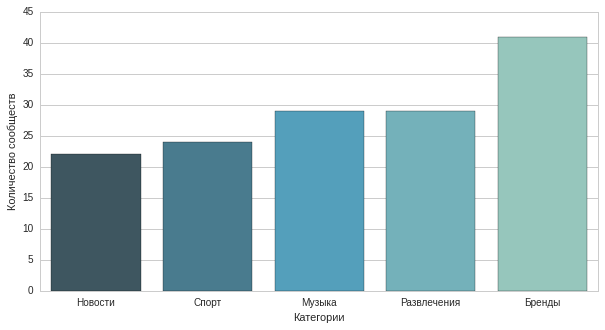
\includegraphics[width=400px]
		{imgs/GroupInCat.png}
		\caption{Количество сообществ в категориях}
		\label{fig:groupincat}
	\end{figure} 
	
	
	\begin{figure}
		\centering
		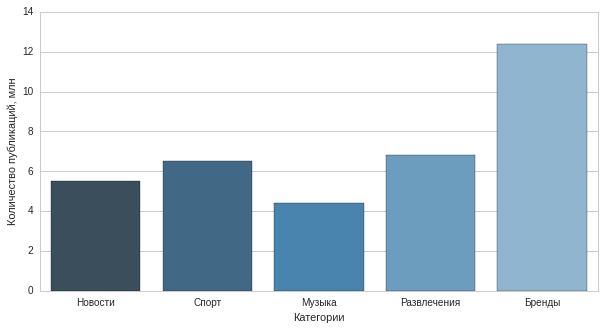
\includegraphics[width=400px]
		{imgs/NumArticles.png}
		\caption{Количество публикаций в категориях}
		\label{fig:numart}
	\end{figure} 
	
В результате для каждого сообщества был создан файл, на первой строке которого записаны идентификатор и название сообщества, а на следующих строках публикации этого сообщества (на одной строке одна публикация).

	\begin{figure}
		\centering
		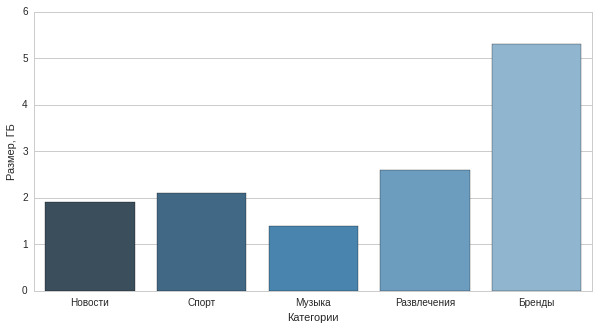
\includegraphics[width=400px]
		{imgs/SizeCat.png}
		\caption{Общий размер публикаций для каждой категории}
		\label{fig:sizecat}
	\end{figure} 
	
	
	
	
	
	
	\subsection{1.3 Предварительная обработка данных}
	Перед тем как приступить к построению тематической модели необходимо провести предварительную обработку данных. 
	Она необходима для того, чтобы избавиться от информации, которая не несет никакой смысловой нагрузки, а следовательно не оказывает заметного влияния на искомые тематики и концепции. 
	Также предварительную обработка включает в себя уменьшение числа форм слов в тексте, в виду того, что обилие различных форм слова ведет к росту словаря и снижению качества модели.
	
	В данной работе полагается, что к информации, которая не несет смысловой нагрузки относятся знаки препинания, эмотиконы \cite{bib:smiley}, гиперссылки и другие символы, не являющиеся цифрами или элементами русского или английского алфавитов. Также к такой информации можно отнести часто используемые слова (стоп-слова): предлоги, местоимения, союзы, числительные и частицы\cite{bib:InformationRetrieval}.
	Стоит отметить, что многие популярные группы связаны друг с другом и имеют одинаковые публикации. А значит возникает проблема дупликатов. В данной работе эта проблема решается с помощью хеш-функций, вычисляемых для текста каждой публикации. \textbf{Нужно ли писать о хеш функциях?}
	
	
	Сокращение числа форм слов в тексте достигается путем применения стемминга или лемматизации к словам. Алгоритм стемминга заключается в поиске неизменяемой части слова, в то время как алгоритм лемматизации более сложен и необходим для поиска нормальной формы слова. Нормальной формой слова в русском языке считается: для существительных~--- единственное число, именительный падеж; для глаголов и причастий~--- глагол в форме инфинитива; для прилагательных~--- мужской род, единственное число, именительный падеж. Как правило, для предварительной обработки текста выбирается один из этих алгоритмов: для русских текстов наиболее эффективна лемматизация, для английских текстов --- стемминг \cite{bib:Voron1}. В виду того, что в данной работе рассматриваются публикации сообществ русскоязычной социальная сети, предпочтение отдается алгоритмам лемматизации.
	
	 
	
	Для предварительной обработки данных был реализован программный модуль на языке Python 2.7. Среди средств для лемматизации были рассмотрены 2 морфологических анализатора из программных пакетов pymorphy2 \cite{bib:pymorphy2} и pymystem3 \cite{bib:pymystem3}. 
	
	Морфологические анализатор представляют собой набор алгоритмов для сопоставления слов и их форм и выявления грамматических характристик слов. В данной работе с помощью морфологических анализаторов осуществляется приведение слов к их нормальной форме.
	
	В результате экспериментов выяснилось, что морфологический анализатор из пакета pymystem3 более эффективен, так как для определения нормальной формы слова учитываются окружающие его слова. Данный функционал отсутствует у морфологического анализатора из pymorphy2, поэтому в реализации данного программного модуля предпочтение было отдано морфологическому анализатору из пакета pymystem3.
	
	
	
	Работа программного модуля заключается в просмотре всех файлов полученных в пункте 1.2. 
	В каждом файле последовательно считываются строки (текст публикации). Для каждой строки вычисляется хеш-функция, значение которой сравнивается со значениями хеш-функций уже просмотренных строк. Если такое значение уже было, то строка удаляется, иначе сохраняется значение хеш-функции. \textbf{(стоит ли писать про асимптотическую сложность, и про хранение значений хешей?)}
	Далее строка обрабатывается морфологическим анализатором. Результатом обработки является строка, в которой все слова приведены к нормальной форме.
	Полученная строка разбивается на подстроки по пробельному символу, после чего каждая подстрока проходит проверку и обработку, в результате чего она либо удаляется, либо заменяется на результат обработки. Из оставшихся подстрок формируется новая строка, которая и будет результатом предварительной обработки.
	
	Алгоритм обработки и проверки подстроки принимает на вход подстроку. \textbf{тут тоже алгоритм, нужно ли описывать его?}
	
	\textbf{стоит ли привести пример работы программного модуля?}
	
	\textbf{Разбиение на тестовую и обучающую выборки}
	\newpage
	\subsection{1.4 Результаты} 
	
	В результате предварительной обработки данных число публикаций значительно уменьшилось. Также пропала одна из категорий сообществ <<Развлечения>>. Это связано с тем, что публикации в данной категории сообществ точно такие же, как и в сообществах других категорий. На рисунке \ref{fig:numart1} изображен график количества публикаций после предварительной обработки. Общее число публикаций уменьшилось с 34 миллионов до 700 тысяч. Также предварительная обработка данных повлияла объем необходимой памяти для хранения публикаций. На рисунке \ref{fig:sizecat1} изображен график, на котором указан объем занимаемой памяти каждой из категорий. Общий объем занимаемой памяти уменьшился с 13 ГБ до 250 МБ.
	
	
	\begin{figure}
		\centering
		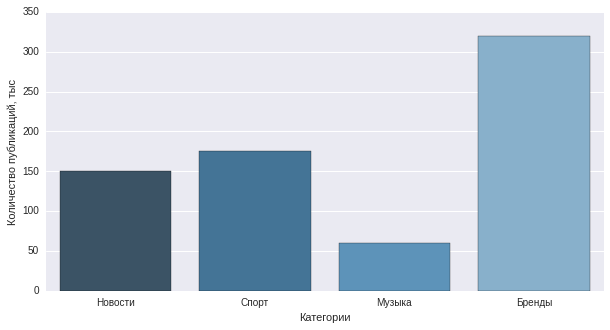
\includegraphics[width=400px]
		{imgs/NumArticles1.png}
		\caption{Количество публикаций в категориях}
		\label{fig:numart1}
	\end{figure} 
	


	\begin{figure}
		\centering
		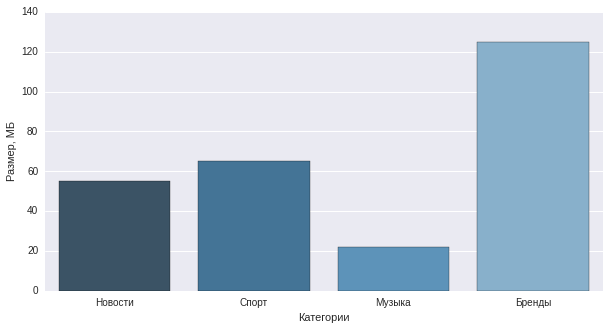
\includegraphics[width=400px]
		{imgs/SizeCat1.png}
		\caption{Общий размер публикаций для каждой категории}
		\label{fig:sizecat1}
	\end{figure} 
	
	
	
	\newpage
	\section{Глава 2. Выбор и построение тематической модели}
	\subsection{2.1 Тематическое моделирование}
	\subsubsection{2.1.1 Основные сведения}
	Тематическое моделирование представляет собой  способ построения тематической модели для коллекции текстовых документов. Построенная тематическая модель предоставляет информацию о тематиках каждого документа и о множестве слов, образующих каждую тематику. 
	
	Тематические модели применяются в задачах тематического поиска, для построения рекомендательных систем, для выявления тематик и концепций в новостных потоках, а также для классификации и кластеризации документов. 
	
	В последнее время широкое распространение получили вероятностные тематические модели, которые основаны на том, что документ или термин может одновременно принадлежать разным тематикам. Вероятностная тематическая модель представляет документы в виде дискретного распределения на множестве тематик, а тематики в виде дискретного распределения на множестве терминов. Такая модель решает проблему синонимии и полисемии. (\textbf{Нужно ли указать каким образом решает?})
	
	\subsubsection{2.1.2 Постановка задачи вероятностного тематического моделирования}
	
	Пусть $D$ --- множество текстовых документов, $W$~--- множество терминов, употребляемых в них. Под термином понимается либо отдельное слово, либо словосочетание. Каждый документ $d \in D$ представлен последовательностью терминов 
	$ \{w_i\}_{i=1}^{n_d}$ из $W$.
	Один и тот же термин может встречаться в документе несколько раз.
	
	Пусть $Z$ - это конечное множесто тематик. Положим, что появление термина $w$ в каждом документе $d$ связано с некоторой, вообще говоря, неизвестной тематикой $z \in Z$. Пользуясь этим представим множества документов в виде множества троек вида $(d,w,z)$, выбранных случайно и независмо из дискретного распределения $p(d,w,z)$, которое задано на множестве $D \times W \times Z$. Независимость элементов выборки подразумевает, что порядок терминов в документе не важен для выявления тематик. Такое предположение носит название гипотезы "мешка слов".
	
	Теперь задачу вероятностного тематического моделирования можно определить следующим образом: построить вероятностную тематическую модель для коллекции документов $D$~--- значит определить множество тематик $Z$, распределения $p(w|z)$ для всех тематик $z \in Z$ и распределения $p(z|d)$ для всех документов $d \in D$.
	
	\subsubsection{2.1.3 Порождающая вероятностная модель}

	Помимо рассмотренных выше гипотез также используется гипотеза об условной независимости, которая указывает на то, что вероятность появления термина $w$ при	условии того, что выбрана тематика $z$ описывается распределением $p(w|z)$ и не зависит от документа $d$. Это эквивалентно следующим равенствам:
	\begin{equation}
		\begin{array}{c c}
			p(w|d,z) = p(w|z); \\
			p(d,w|z) = p(d|z)p(w|z)
		\end{array}
	\end{equation}

	Используя гипотезу условной независимости и определяния условной и полной вероятности получаем
	
	\begin{equation}
		p(w|d) = \sum_{z \in Z} p(w|z)p(z|d).
	\label{eq:pwd}
	\end{equation}
	
	Равенство (\ref{eq:pwd}) описывает процесс порождения множества документов $D$, если известны распределения $p(w|z)$ и  $p(z|d)$. Задача при построении тематической модели наоборот найти распределения $p(w|z)$ и  $p(z|d)$ по известному множеству документов $D$.
	
	\subsection{2.2 Выбор тематической модели}
	
	Рассмотрим две вероятностные тематические модели pLSA и LDA, и сравним их. 
	Для начала введем следующие обозначения:
	
	\begin{equation}
		\begin{array}{l l}
			
			\Phi = (\varphi_{wz})_{|W| \times |Z|}, & \quad
				\varphi_{wz} = p(w|z); \\
			\Theta = (\vartheta_{zd})_{|Z| \times |D|}, & \quad
				\vartheta_{zd} = p(z|d).
		\end{array}
		\label{eq:desc}
	\end{equation}
	где $\Phi$~--- матрица терминов тематик, а $\Theta$ - матрица тематик документов. Стоит обратить внимание на то, что матрицы $\Phi$ и $\Theta$ являются стохастическими. Под стохастическом матрицей понимается матрица с нормированными столбцами и неотрицательными элементами.
	
	Модели pLSA и LDA основаны на вероятностной модели появления пары <<документ-слово>>,  которая может быть представлена следующим образом:
	
	\begin{equation}
	p(d,w) = \sum_{z \in Z}p(w|z) p(z|d) p(d),
	\label{eq:pmodel}
	\end{equation}
	где $p(d)$ --- это априорное распределение на множестве документов.
	
	
	\begin{figure}
		\centering
		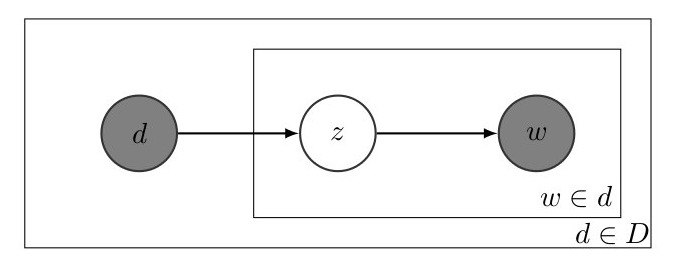
\includegraphics[width=400px]
		{imgs/PLSA.jpg}
		\caption{Байесовская сеть модели pLSA}
		\label{fig:plsa}
	\end{figure} 
	
	
	\subsubsection{2.2.1 Вероятностое латентно-семантическое моделирование}
	Модель pLSA можно представить в виде Байесовской сети, изображенной на рисунке \ref{fig:plsa}. Байесовская сеть представляет собой ориентированный ацикличный граф, вершинами которого соответствую случайным переменным, а ребра соответсвуют распределениям условной вероятности, где родительский узел сооветствует условной переменной, а дочерний --- зависимой переменной. Темные вершины на графе соответстсуют наблюдаемым переменным (их значения известны), а белые вершины соответствуют латентным переменных, значение которых нужно найти. Для модели pLSA наблюдаемыми переменными будут $d$  и $w$, а латентной~--- переменная $z$. Переменная $d$ хранит индекс документа, $w$ - индекс слова, $z$ - индекс темы. Прямоугольник, включающий в себя некоторый подграф $\mathbf{G}$, обозначает набор из нескольких экземпляров подграфа $\mathbf{G}$. Число экземпляров определяется надписью в правом нижнем углу прямоугольника.
	\cite{bib:Heinrich}. 
	
	В pLSA для оценивания параметров по коллекции документов $D$ используется принцип максимума правдоподобия, который приводит к задаче максимизации следующего функционала:
	
	\begin{equation}
		\begin{array}{c c}
		\mathlarger{ 
			\sum_{d \in D} 
			\sum_{w \in d}
			n_{dw} 
			\ln \sum_{t \in T}
			\varphi_{wt} \vartheta_{td} 
			\rightarrow \max_{\Phi, \Theta};
			} \\
		\mathlarger{
			\sum_{w \in W} \varphi_{wt} = 1; \quad \sum_{t \in T} \vartheta_{td} = 1.
		}
		\end{array}
	\label{eq:maxtask}
	\end{equation}
	где $n_{dw}$~--- это число упомнинаний термина $w$ в документе $d$.
	
	Обычно для решения задачи (\ref{eq:maxtask}) используется EM-алгоритм, принцип работы  которого рассмотрен в приложении.
	
	Основные недостатки модели pLSA:
	\begin{itemize}
	\item{Число параметров линейно зависит от числа документов в коллекции, что ведет к переобучению модели.}
	\item{Невозможно вычислить $p(t|d)$ для документа $d$, если он был добавлен в коллекцию после построения модели. \cite{bib:Voron1}  }
	\end{itemize}
	
	
	\subsubsection{2.2.2 Латентное размещение Дирихле}
	
	Как и в pLSA в основе LDA лежит вероятностная модель (\ref{eq:pmodel}), но теперь делаются дополнительные предположения о том, что 
	векторы документов $\vartheta_d = (\vartheta_{dz}) \in \mathbb{R}^{|T|}$ 
	и 
	векторы тематик $\varphi_z = (\varphi_{wz}) \in \mathbb{R}^{|W|}$ 
	порождаются распределениями Дирихле с параметрами 
	$ \alpha \in \mathbb{R}^{|T|} $ 
	и
	$ \beta \in \mathbb{R}^{|W|} $ соответственно:
	
	$$  \mathlarger{
		\text{Dir}(\vartheta_d; \alpha) = 
		\dfrac
			{ \Gamma(\alpha_0)			}
			{ \prod \limits_z \Gamma (\alpha_z) }
		\prod_z \vartheta_{zd}^{\alpha_z - 1}
		},
		\alpha_z > 0, 
		\alpha_0 = \sum_z \alpha_z,
		\vartheta_{zd} > 0, 
		\sum_z \vartheta_{zd} = 1;		
	$$
	$$  \mathlarger{
		\text{Dir}(\varphi_z; \beta) = 
		\dfrac
			{ \Gamma(\beta_0)			}
			{ \prod \limits_w \Gamma (\beta_w) }
		\prod_w \varphi_{wz}^{\beta_w - 1}
		},
		\beta_w > 0, 
		\beta_0 = \sum_w \beta_w,
		\varphi_{wz} > 0, 
		\sum_w \varphi_{wz} = 1;		
	$$
	где $\Gamma (z) $~--- гамма-функция.
	
	Учитывая данные предположения рассмотрим Байесовскую сеть модели LDA, изображенную на рисунке \ref{fig:lda}. Параметры $\alpha$ и $\beta$ являются гиперпараметрами моделями и параметрами распределения Дирихле, и, как правило, задаются до начало обучения модели. Переменная $w_{n,d}$ является наблюдаемой и представляет собой индекс $n-го$ слова в документе $d$. Все остальные переменные являются латентными (скрытыми).
	
	Для оценки параметров модели LDA по коллекции документов $D$ вариационный Байесовский вывод, метод сэмплирования Гиббса или метод Expectation-Propagation.
	
	Основной недостаток модели LDA заключается в том, что априорные распределения Дирихле не моделирует никаких особенностей языка и имеют слабые лингвистические обоснования. Они используются для того, чтобы облегчить баесовский вывод для модели \cite{bib:Voron1}
	
	
	
	\begin{figure}
		\centering
		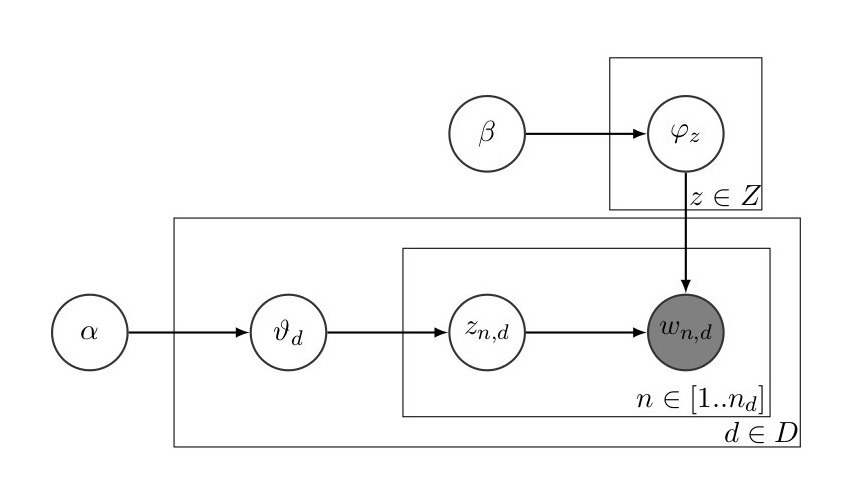
\includegraphics[width=400px]
		{imgs/LDA.jpg}
		\caption{Байесовская сеть модели LDA}
		\label{fig:lda}
	\end{figure} 
	
	
	\subsubsection{2.2.3 Вывод}
	Учитывая количество публикаций полученных из социальных сетей, достоинства и недостатки рассмотренных моделей разумным будет выбрать тематическую модель LDA. Выбор LDA облегчит работу с обучающей и тестовой выборками публикаций, так как для проверки работы модели на тестовых данных не придется выполнять построение модели заново.  Также стоит обратить внимание на то, что модель pLSA больше подвержена переобучению, чем модель LDA.
	
	В качестве метода для оценки параметров модели приоритет был отдан сэмплированию Гиббса,  так как этот метод является относительно простым и эффективным алгоритмом для решения задач статистического оценивания. \textbf{[обосновать подробнее?]}

	\subsection{2.3 Построение тематической модели}
	
	Выбранная вероятностная тематическая модель LDA была реализована в виде программного модуля на языке программирования  С++. 
	
	\subsection{2.5 Эксперименты}
	
	
	\newpage
	\section{Глава 3. Оценка качества модели}
	\subsection{3.1 Обзор оценок качества тематических моделей}
	\subsection{3.2 Оценка качества построенной тематической модели}
	
	
	\newpage
	\section{Анализ результатов}
	
	
	\newpage
	\section{Заключение}
	
	
	
	\newpage
	\section{Список литературы}
	
    \begingroup
    \let\clearpage\relax
    \vskip-3cm
	\begin{thebibliography}{9}
	
		\bibitem{bib:Kaklauskas}
		Arturas Kaklauskas. Biometric and Intelligent Decision Making Support // Springer, 2015, P. 220.
		
		\bibitem{bib:Paul}
		Paul, MJ. and M. Dredze. You Are What You Tweet: Analyzing Twitter for Public Health. // In Proc. of the 5th International AAAI Conference on Weblogs and Social Media (ICWSM),  2011. 
		
		\bibitem{bib:InformationRetrieval}
		Christopher D. Manning, Prabhakar Raghavan and Hinrich Schütze. Introduction to Information Retrieval. Cambridge University Press, 2008. 506 P.
		%\bibitem{bib:DataMining}
		%Pang-Ning Tan, Michael Steinbach and Vipin Kumar. Introduction to Data Mining. Addison-Wesley, 2006. 769 P.	
		%\bibitem{bib:Seragan}
		%Toby Segaran. Programming Collective Intelligence. O'Reilly Media, 2007. 362 P.
		
		\bibitem{bib:Hoffman}
		Thomas Hofmann. Probabilistic latent semantic indexing. Proceedings of the Twenty-Second Annual International SIGIR Conference, 1999.
		
		\bibitem{bib:Blei}
		David M. Blei, Andrew Y. Ng, Michael I. Jordan. Latent Dirichlet Allocation // Journal of Machine Learning Research 3, 2003. P.~993~--~1022.
		
		\bibitem{bib:Heinrich}
		Gregor Heinrich. Parameter estimation for text analysis. Technical
report, Fraunhofer IGD, Darmstadt, Germany, 2005.

		\bibitem{bib:Blei2}
		David Blei. Introduction to Probabilistic Topic Models // Communications of the ACM, 2012. P. 77–84.

		\bibitem{bib:Voron1}
		Воронцов К.В. Вероятностное тематическое моделирование // www.machinelearning.ru : web. — 2013.

		\bibitem{bib:Popularity}
		http://www.statista.com/statistics/278414/number-of-worldwide-social-network-users/

		\bibitem{bib:PopularNetwork}
		http://www.statista.com/statistics/272014/global-social-networks-ranked-by-number-of-users/
		
		\bibitem{bib:vkapi}
		API Vkontakte: https://vk.com/dev/apiusage
		
		\bibitem{bib:methods}
		Описание методов API Vkontakte: https://vk.com/dev/methods
		
		\bibitem{bib:smiley}
		https://ru.wikipedia.org/wiki/Эмотикон
		
		\bibitem{bib:pymorphy2}
		Документация для морфологического анализатора pymorphy2: https://pymorphy2.readthedocs.io/en/latest/
	
	
		\bibitem{bib:pymystem3}
		Документация для pymystem3: https://pypi.python.org/pypi/pymystem3/0.1.1
		
		\bibitem{bib:ml}
		ссылка на machine learning
		
		\bibitem{bib:doc}
		можно всякие документации добавить

	
		
		

		
		
		%%% Примеры
		%%% КНИГА ОДНОГО АВТОРА
		%\bibitem{bib:Viner}
		%Винер~В. Нелинейные задачи в теории случайных процессов.~М.:~ИЛ,~1961. 159~с.
		
		%%% КНИГА НЕСКОЛЬКИХ АВТОРОВ
		%\bibitem{bib:Demidovich}
		%Демидович~Б.\:П., Марон~И.\:А., Шувалова~Э.\:З. Численные методы анализа. Приближение функций, дифференциальные и интегральные уравнения.~М.:~Наука,~1967. 368~c.
		
		%%% СТАТЬЯ В ЖУРНАЛЕ
		%\bibitem{bib:Nadaraya} 
		%Надарая~Э.\:А. Об оценке регрессии // Теория вероятностей и ее применения, 1964. Т.~9, Вып.~1. С.~157~--~159.
		
		%\bibitem{bib:Sinitzin}
		%Синицын~И.\:Н. Методы статистической линеаризации (обзор) // АиT,~1974. №~5. С.~82~--~94.
		
		%\bibitem{bib:Billings}
		%Billings~S.\:A., Fadzil~M.\:B., Sulley~J., Johnson~P.\:M. Identification of a nonlinear difference equation model of an industrial diesel generator // Mechanical Systems and Signal Processing,~1988. Vol.~2, No~1. P.~59~--~76.
		
		%\bibitem{bib:Bouton}
		%Booton~R.\:C. Nonlinear control systems with random inputs // Trans. IRE Profes. Group on Circuit Theory,~1954. Vol.~CT1, No~1. P.~9~--~18.
		
		%\bibitem{bib:Boyd}
		%Boyd~S., Chua~L.\:O. Fading memory and the problem of approximating nonlinear operators with Voltterra series // IEEE Trans. Circuits Syst.,~1985. Vol.~CAS-32, No~11. P.~1150~--~1161.
		
		%\bibitem{bib:Gagarin}
		%Garain~U. Identification of mathematical expressions in document images // Proc. of the 10th Int. Conf. on Document Analysis and Recognition (ICDAR),~2009. P.~1340~--~1344.
		
		%\bibitem{bib:Lee}
		%Lee~H.\:J., Wang~J.\:S. Design of a mathematical expression understanding system // Pattern Recognition Letters,~1997. Vol.~18, No~3, P.~289~--~298.
		
		
		
		%\bibitem{Steinberg}
		%Штейнберг~Ш.\:Е. Идентификация в системах управления.~М.:~Энергоатомиздат,~1987. 80~с.
		
		% \bibitem{bib:Petrov}
		%Петров~Л.\:И. О культуре набора текста на ПМ–ПУ.~СПб:~Изд. дом C.-Петерб. ун-та,~1726. 324~c.
		
		
		
		%\bibitem{bib:Kalitkin}
		%Калиткин~Н.\:Н. Численные методы.~М.:~Наука,~1978. 512~c.
		
		%\bibitem{bib:Berezin}
		%Березин~И.\:С., Жидков~Н.\:П. Методы вычислений. Том~1. Изд.~2-е, стереотип.~М.:~ГИЗ ФИЗМАТЛИТ,~1962. 464~c.
		
		%%% КНИГА ПОД РЕДАКЦИЕЙ
		%\bibitem{bib:Reibmann1}
		%Дисперсионная идентификация / Под ред. Н.\:С.~Райбмана.~М.:~Наука,~1981. 320~с.
		
		%%% СТАТЬЯ В СБОРНИКЕ
		%\bibitem{bib:Vlasov}
		%Власов~С.\:А., Шплихал~Й. Состояние разработок и перспективы развития имитационных систем для анализа функционирования и автоматизированного проектирования производства (на примерах металлургии и машиностроения) // Моделирование и идентификация 		производственных систем.~М.:~Институт проблем управления,~1988. С.~5~--~17.
		
		%\bibitem{bib:Reibmann2}
		%Райбман~Н.\:С. Методы нелинейной и минимаксной идентификации // Современные методы идентификации систем / Под ред. П.~Эйкхоффа.~М.:~Мир,~1983. С.~177~--~277.
		
		%\bibitem{bib:Bure:29}
		%Буре~В.\:М., Кирпичников~Б.\:К. Оптимальные решения по выборочным данным // Процессы управления и устойчивость: Труды 29-й научной конференции / Под ред. В.\:Н.~Старкова.~СПб.:~НИИ Химии СПбГУ,~1998. С.~296~--~299.
		
		%\bibitem{bib:Bure:32}
		%Буре~В.\:М. Кооперативное решение в задаче перестрахования риска // Процессы управления и устойчивость: Труды 32-й научной конференции студентов и аспирантов факультета ПМ-ПУ / Под ред. В.\:Н.~Старкова.~СПб.:~ООП НИИ Химии СПбГУ,~2001. С.~396~--~398.
		
		%%% ССЫЛКА НА ДОКУМЕНТ В ИНТЕРНЕТЕ		
		%\bibitem{bib:LAM} 
		%LAM/MPI Parallel Computing. http://en.wikibooks.org/wiki/LaTeX
		
		%\bibitem{bib:Latex}
		%LaTeX on Wikibooks. http://en.wikibooks.org/wiki/LaTeX
		
	\end{thebibliography}
    \endgroup
	%%\section{*Приложение}
	%%Приложи сюда свой код	
\end{document}